\documentclass{standalone}
\special{background White}

\usepackage{tikz}
\usepackage{caption}
\usepackage{subcaption}
\usepackage{graphicx}
\begin{document}

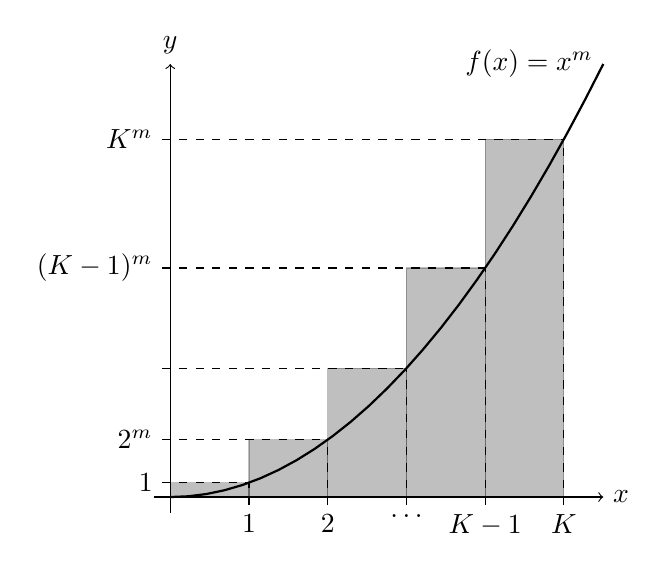
\begin{tikzpicture}[domain=0:5.5, scale=1]
    \tikzset{declare function={f(\x)=\x^2/5.5;}} %% define function
    % \draw[very thin,color=gray] (0,0) grid (8,8);

    \draw[->] (-0.2,0) -- (5.5,0) node[right] {$x$};
    \draw[->] (0,-0.2) -- (0,5.5) node[above] {$y$};

    \draw[thick]    plot (\x,{f(\x)})   node[left] {$f(x) =x^m$};

    \foreach \x/\xtext/\ytext in {1/1/1,2/2/2^m,3/\dots/ ,4/K-1/(K-1)^m,5/K/K^m} {
            \draw[dashed] (\x,-0.1) node[below] {$\xtext$} -- (\x,{f(\x)}) ;
            \draw[dashed] (-0.1,{f(\x)}) node[left] {$\ytext$} -- (\x,{f(\x)});
            \filldraw [black, nearly transparent] ({\x-1},0) rectangle (\x,{f(\x)});
        }
\end{tikzpicture}
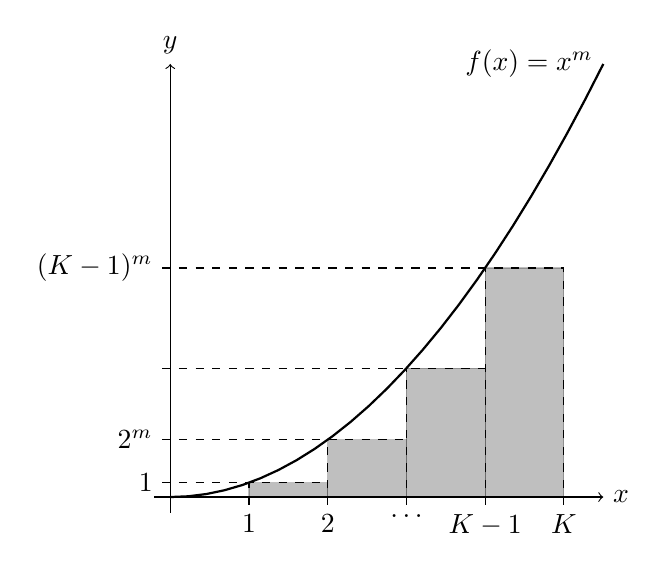
\begin{tikzpicture}[domain=0:5.5, scale=1]
    \tikzset{declare function={f(\x)=\x^2/5.5;}} %% define function
    % \draw[very thin,color=gray] (0,0) grid (8,8);

    \draw[->] (-0.2,0) -- (5.5,0) node[right] {$x$};
    \draw[->] (0,-0.2) -- (0,5.5) node[above] {$y$};

    \draw[thick]    plot (\x,{f(\x)})   node[left] {$f(x) =x^m$};

    \foreach \x/\xtext/\ytext in {1/1/1,2/2/2^m,3/\dots/ ,4/K-1/(K-1)^m} {
            \draw[dashed] (\x,-0.1) node[below] {$\xtext$} -- (\x,{f(\x)}) ;
            \draw[dashed] (-0.1,{f(\x)}) node[left] {$\ytext$} -- ({\x+1},{f(\x)});
            \filldraw [black, nearly transparent] ({\x},0) rectangle ({\x+1},{f(\x)});
        }
    \draw[dashed] (5,-0.1) node[below] {$K$} -- (5, {f(4)});
\end{tikzpicture}

\end{document}